
\sectionnotitle
\section{女子寮生座談会}\label{sec:josiryose}
\sectiondefault


\begin{figure}[H]
  \centering
  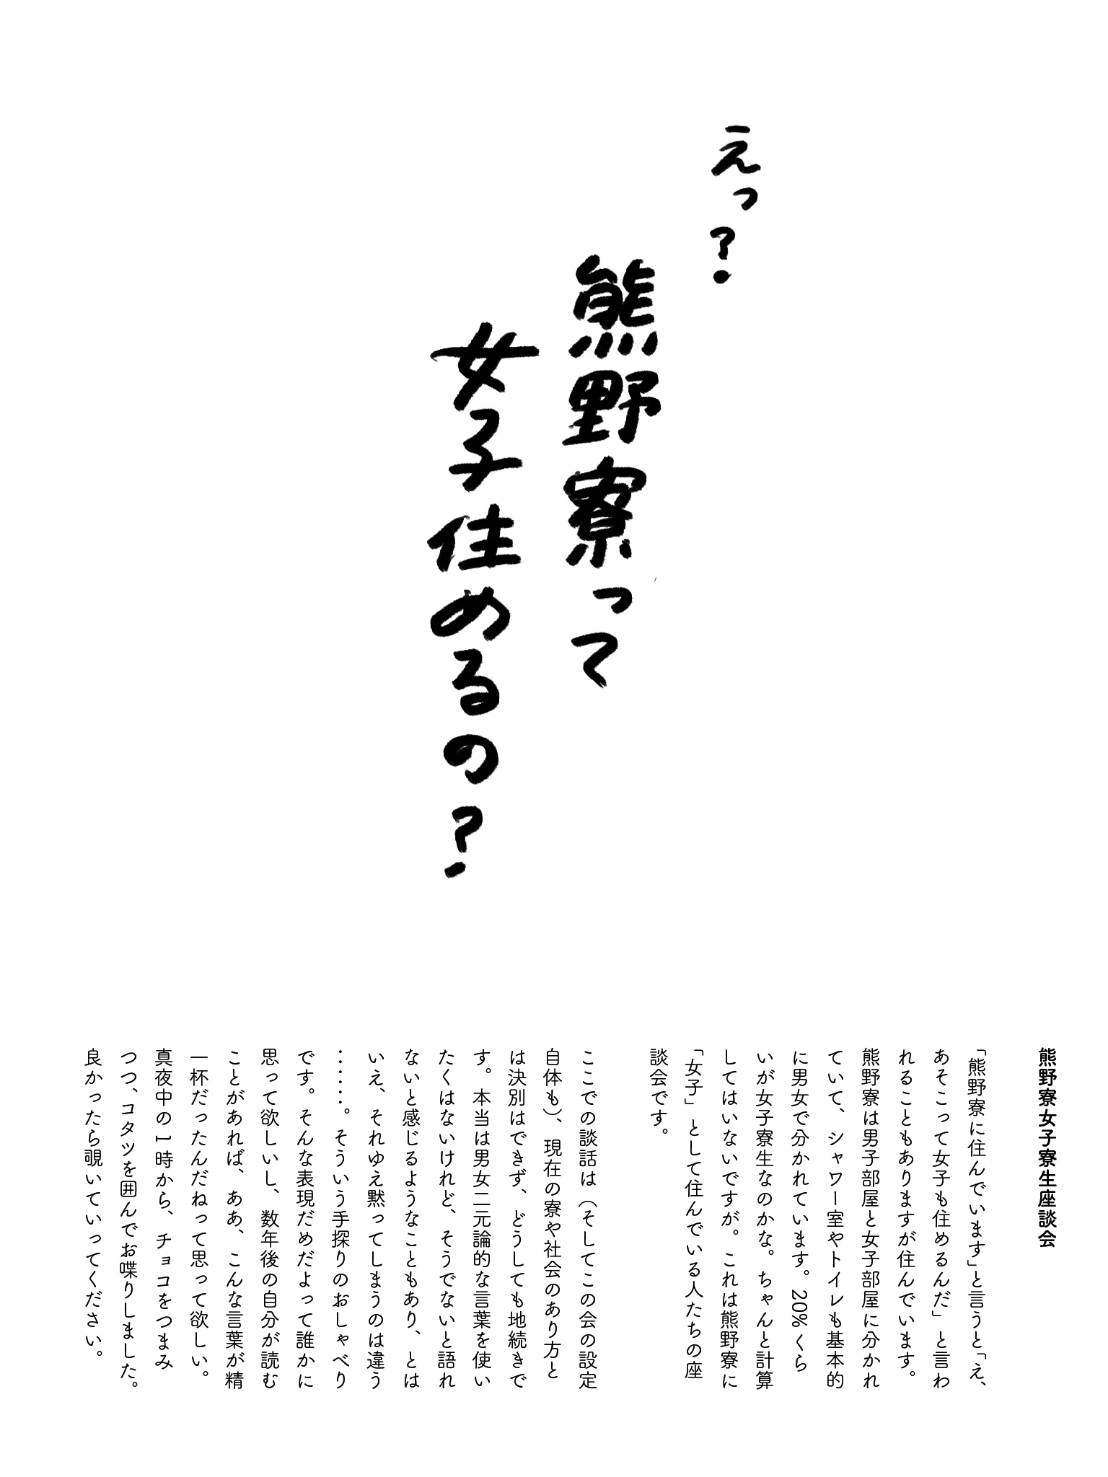
\includegraphics[width=18cm]{gazo/josiryose_title.jpg}
\end{figure}

\newpage


\begin{figure}[H]
  \centering
  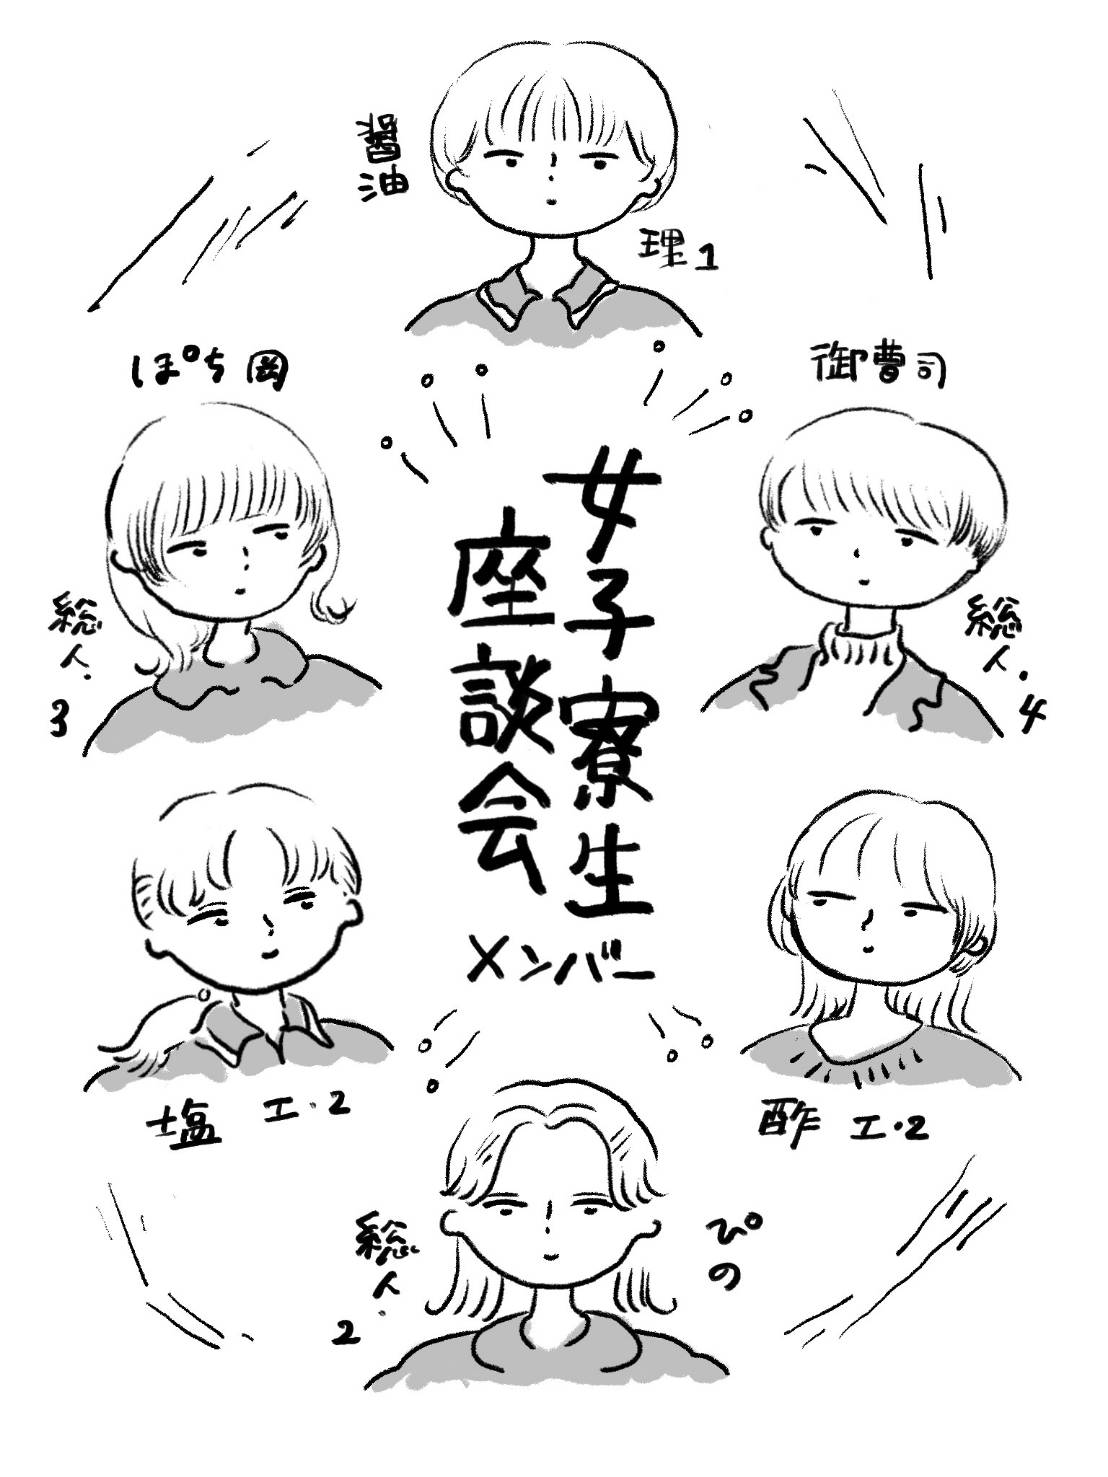
\includegraphics[width=18cm]{gazo/josiryose_member.jpg}
\end{figure}

\newpage




\begin{multicols}{2}

\subsection{参加者紹介}


\begin{boxnote}
  
    酢:入寮2年目。絵が上手。櫓が好き。

    御曹司:入寮4年目。4回生後期から休学中。

    ぴの:入寮2年目。歌が上手。人間が好き。

    醤油:入寮1年目。料理がうまい。生麩が好き。

    塩:入寮2年目。好きなものは食べ物。

    ぽち岡:入寮3年目。寮の喫煙所が好き。
  
\end{boxnote}





  \talker{酢}座談会始めて行きましょう。

  去年も喋ってた話題で、寮で女性が暮らしやすいかとか、生活面で困ったことがあるかみたいな話と、あと京大の中で女子ってどんな感じで過ごしてるのかということ。あと去年はあんまり話さなかったんですけど女子寮生個人の人となりがわかったら入る人も安心するのかなと思って、寮でこういう活動してますとか、こういうことが好きですみたいなことをしゃべろうかなって感じです。あと女子寮生新歓設立の経緯とかを、ぽち岡さん中心に聞いていきたいなと。

  最初、自己紹介から始めましょう。







  \subsection{自己紹介}





  \talker{酢}学部は工学部、学科は建築で2回生です。寮では1回生のときから広報局というところに所属して、寮の広報をしたり寮で作る冊子とかのデザインを作ったりしています。あと、熊野寮ではまだ建ててないけど吉田寮で櫓を以前建てて、今後も建築物を寮に増やしていきたいと思っています。



  \talker{御曹司}総合人間学部4回生で、寮ではあんまり何もやってない...。MUC\footnote{Music room Users' Conferenceの略。熊野寮にある音楽室を維持、管理する会議体。音楽室利用者会議。}でギターを弾いたり...よく寝ています。1年の終わりの実家に帰ってるタイミングでめちゃめちゃコロナが流行り始めて、寮内の人口密度を減らすために一旦みんな実家に疎開してくださいっていうことがあって、それで丸1年実家に帰っていました。だから寮生活は実質のべ3年目ですね。



  \talker{ぴの}総合人間学部2回生です。寮では主にMUCの活動をやっていて、その中でもとりわけC棟、同回生、入寮当初からのバンドであるShe is Cにコミットしています。他にはつい先日のNF公演でKMN48\footnote{熊野寮を拠点に自治やっちゃう系アイドルとして活動する、AKBグループのコピーダンスユニット。性別、寮籍問わずメンバー募集中!}のメンバーとしてステージデビューをさせていただきました。



  \talker{醤油}理学部1回生です。寮で何をしているか...何もしてないですね。寮自治を甘噛みして、最近は食北という食堂北部にあるスペースを拡大するという計画にすごく力を注いでいます。そしてこのこたつでずっと寝ていて、大学にはほとんど行ってないです。そんな感じでやってます。日が昇る頃に寝て15時ぐらいに起きてダラダラするという生活を日々過ごしています。系登録\footnote{理学部において数学系、物理系、化学系、生物系、地学系のいずれかに配属されること。一定の単位や成績をそろえないと系登録はできない。}したいよーわんわん。



  \talker{塩}工学部地球工学科の2回生です。何をしてるかと言われたらKUMANですね。地域の子供たちに勉強を教えたり一緒に遊んだりとかを近くの集会所でやる無料の寺子屋みたいなのをやっています。寮祭で動物園に行く企画をやって楽しかったです。ここ半年の目標は立派な猛獣使いになることです。



  \talker{ぽち岡}総合人間学部の3回生です。寮では主に寮生の人権を守っています(この1年はあまり守れませんでした...。ごめんな)女子寮生新歓という企画を運営したり、女子寮生向けハラスメント相談窓口という組織をギリギリ生きながらえさせたりしています。普段は、KMN48が天下を取れるように頑張っています。あとは日々部屋を散らかしています。



  \subsection{大学での生活}



  \talker{酢}まずは大学での生活について話そうかなと思っています。受験生がまず知りたいのは京大で女子ってどんな感じで暮らしてるかっていうことかなと思ったので。ちょうど理系3、文系3だし。

  \talker{ぽち岡}文系が総人(総合人間学部)しかいない。

  \talker{酢}確かに、みんな総人。じゃあとりあえず総人から、女子の比率とか、何かこんなことがありましたとかあったら。

  \talker{ぽち岡}総人...どうだろう

  \talker{ぴの}半々よりは若干男子の方が多いかな。

  \talker{ぽち岡}文学部、教育学部の次ぐらいに女子多いイメージ。半分弱。私の代は、入学して今年入学の人みたいなLINEグループができるときに総人女子っていうグループができて、そこで女子会をやったりしてた。私は日和って参加してなかったから友達が2人しかいません(笑)

  \talker{酢}2人もいるんだすごい。

  \talker{ぽち岡}総人、女子結構元気。のびのびしてるイメージがあります。

  \talker{御曹司}19年度入学にもありましたね、学年全体の総人女子グループ。なんかやってたっけ。ちょっと見てみます。

  \talker{酢}総人って入学式のあと交流会みたいなのやってますよね。

  \talker{御曹司}そうね。

  \talker{塩}前は合宿とかやってませんでした?大学の冊子に載ってた覚えがある。

  \talker{御曹司}やってました。やってました。なんかね総人入学当初にうちのクラスの担任が言ってたんだけど、必修の授業とかで他の学部に比べて一緒に受ける機会が全くないから「総人のクラスなんてあってないようなもんだから今のうちに仲良くしときなね」って。合宿の時に。

  \talker{ぴの}実際2回生に上がってから、ライリス\footnote{京大の一般教養科目「英語ライティングーリスニング」の略。大体の場合、この授業の単位を取らないと卒業できない。}とかリーディング\footnote{京大の一般教養科目「英語リーディング」の略。大体の場合、この授業の単位を取らないと卒業できない。}とか唯一の共通科目だった(友人)関係の最後の命綱みたいなのもなくなり、まあ疎遠になるわなるわ。でも寮だからあんまり困ってないけどね思ってしまう。

  \talker{酢}結構女子が多いから別にそんなに少数派感はないのかな。

  \talker{ぴの}確かに

  \talker{ぽち岡}全員少数派みたいな学部だから。

  \talker{酢}専門がバラバラなのか。

  \talker{御曹司}そうっすね。授業もバラバラだし。

  \talker{ぴの}ただ強いて言うなら、興味が似てる人は「あ、またいる!」みたいな感じで出会うことはできる。

  \talker{御曹司}そうっすね。最初の1年で仲良くなる人よりも、後々あれなんかこの人よく見るわっていうので仲良くなる人の方が多い気がする。あれなんか面白い。

  \talker{ぽち岡}総人、学系っていうのが5つあって、ほぼ全員が5つの内の2つに集中するんよ。

  \talker{醤油}残りの3つかわいそう

  \talker{ぽち岡}人間科学系と認知情報学系にみんな行って、残り3つのうち2つに残りがバラバラと入って、自然科学系がめっちゃ少ない。自然科学系に行く女子は超少数派かも。学系によっては他の理系学部と同じような比率になっていくのかもしれないけど、それ以外はそうでもない。



  \talker{塩}工学部女子は少数だよね。

  \talker{醤油}でも建築(学科)と地球工(学科)で違うんじゃないですか。建築の方が多いらしい、今調べたら。

  \talker{酢}建築は3割ぐらい。

  \talker{塩}地球工は2割とか?

  \talker{醤油}なんか2022年のやつは、建築が19\%で地球工が10\%です。

  \talker{塩}少ないな。でも確かに全然いない。クラスによって大学側が女子をかためてくれてて、私のクラスは女子が一番多いクラスなんですけど、女子ゼロのクラスも2つくらいありますね。

  \talker{ぴの}総人って第3外国語まで選べて、中級を受けずに初級に戻ることができるという制度があるんだけど、それでクラス指定じゃない別の外国語でたまたま工学部のクラスに組み込んでいったんだけど、普段の学部の景色と違って30人分の3みたいな。やっぱり10\%という数字の通り。

  \talker{塩}実験とかだいたい女子1人。

  \talker{醤油}わかるー

  \talker{塩}そうだよね。グループに分けられるんですけど。女子一人であることに対して何も思わなくなる。女子っていないよねみたいな感覚になってくる。

  \talker{酢}建築でうちの学年は多分女子25\%ぐらいとかでそんなにめっちゃ少数派って感じはないけど、建築女子みたいなLINEグループがある。

  \talker{塩}地球工はないな。クラスの女子グループはあるけど。クラスの女子は割と仲いいんですよ。全員ちゃんと顔と名前がわかって、ある程度コミュニケーション取れるんですけど…

  \talker{ぽち岡}すげー

  \talker{塩}他のクラスは全然だし、男子との交流も本当になくて、実験で少し話すことはあるけど、授業のとき話さないし、話す必要があることも特にない。

  \talker{酢}建築女子LINEグループがあって、建築学科の全体LINEグループもあるけど、建築男子グループがあるのかないのかはわからない、必要ないのかな。

  \talker{ぽち岡}なんか教育学部男子のLINEグループが話題になってたことなかったっけ?意外と男子グループっていうのもあるんだなって思った記憶がある。

  \talker{塩}工学部で男子グループはなさそう。ほぼみんなだし。

  \talker{ぽち岡}総人だったらありそうな感じする。

  \talker{酢}建築女子(のLINE)グループが何で存在するのかあんまわかってないんですよね。1,2回みんなで同志社パフェ食べに行きましょうみたいなのあったけど、それ以降なんにも…。建築は総人みたいにバラバラになることがなくてみんなほとんど一緒にいて仲良くなるから、あんまり女子で分かれるっていうことがそもそもないかもしれない。段々LINEグループが動かなくなっていった。

  \talker{御曹司}19年度の総人女子のLINEグループを見直してみたんですけど、女子会の企画とかすらなくて、サークルの宣伝とライリスの宿題の話ばっかりしてる。

  \talker{一同}(笑)

  \talker{御曹司}絶対女子である意味ない。

  \talker{塩}大体女子LINEってそんなもんじゃないですか。私もクラスの女子LINE、女子である必要のあること何も言ってない。そこでLINEグループができたからそこで会話してるだけで、学科全体のグループには投下できないからみたいな。

  \talker{醤油}少数でしゃべりやすいからね。

  \talker{ぴの}宿題って本当はできるだけ多くの人に聞いた方が早いけど、でもちょっと全体はなあって時に

  \talker{御曹司}確かに多分そういうことですよね

  \talker{酢}工学部はそんな感じですかね?でも学科による?

  \talker{塩}情報(学科)が1番女子少なくて、電電(電気電子工学科)がその次に少なくて、物工(物理工学科)が多分その次に少なくて、その次が地球工、工化(工業化学科)、建築。

  \talker{ぽち岡}私のブロック、女子の先輩で工化2人いるし。工化は(女子)多いよね。

  \talker{塩}女子の数が成績と相関関係があるのが悔しい。

  \talker{酢}女子が理系科目苦手みたいなのが本当なのか疑問だけど、自分的には先輩で目指す人がいないと、理系目指すってならないのかなって気がしてて…。

  \talker{塩}何かどこかで内面化されちゃってる感じあるよね。バリバリ理系は男子みたいな。

  \talker{ぽち岡}女子で理系って言ったら医療系に多いよね。

  \talker{醤油}確かに人健(医学部人間健康科学科)とか半分ぐらい女子ですよ。

  \talker{塩}医学科も割と多いよね。

  \talker{醤油}2割とかいるはず。

  \talker{ぽち岡}私も親に言われてたもん。女なんだから手に職つけておいた方が良いよって。

  \talker{一同}へー

  \talker{ぽち岡}子供産んで仕事を中断しても医療系の資格なら再就職困らないから、医学部行けみたいなこと言われて、すごい反抗した記憶がある。

  \talker{酢}親に言われてはないんですけど、手に職を付けておいた方がいいのかなっていうのは思ってて、結婚とか出産で中断されるかもしれないって考えたら、資格取れるやつとかがいいよなとやっぱりちょっと思っちゃう。

  \talker{ぽち岡}そう考えざるを得ないよね。

  \talker{御曹司}何も考えてなかった(笑)

  \talker{ぽち岡}薬学部の寮生ってあんまり見なくない?

  \talker{塩}1人会ったことある!

  \talker{酢}再履修で薬学部の線形代数を受けてるけど、女子多い。

  \talker{ぽち岡}薬学部って女子多いイメージあるよね。

  \talker{塩}医療系だから、医学部と似てるところがありそう。

  \talker{ぽち岡}なんか、中学生ぐらいのときにプロフ帳交換したらさ、成績良い女子みんな将来の夢「薬剤師」って書いてて…

  \talker{塩}薬剤師流行りますよね!周りの友達で薬剤師になりたい子何人かいました

  \talker{ぽち岡}流行るよね!身近で働いてる女の人を見る機会が学校の先生、看護師さん、薬剤師さん歯科衛生士さんとかに固定されてるから、勉強してなる仕事ってなったら薬剤師みたいなそういうノリがあった気がする。懐かしいな。みーんなプロフ帳に薬剤師って書いてた。

  \talker{一同}(笑)

  \talker{醤油}私はそもそも全然学部にコミットしてないっていうか、理学部どうなんだろう。わりと授業とかもバラバラだから、総人とかほどじゃないけど、理系にしては色んな系を志望する人がいて、みんな授業割と取るの違うから、クラスで語学と数学の授業はみんな一緒。でも私は授業全然行ってないからあれですけど、私のクラス40人くらいいて、女子は私含めて3人しかいなくて、来ないとすぐわかるんですよ(笑)

  \talker{醤油}しかも女子でマイノリティだから、教室とか入っていくとなんか「およ」って顔される。

  \talker{塩}それわかるかも。数学の授業とか受けてて遅刻して入ると、なんかいつもあいつだみたいな目で見られる。

  \talker{醤油}それは遅刻してるからじゃないですか(笑)

  \talker{塩}いやでもさ、男子だったら多分あんまり特定されないじゃん。絶対特定されてるなっていう確信がある。

  \talker{ぽち岡}女子っていうだけで男子の派手髪のやつと同じ目立ち方になるもんね。スタートラインが。女子で髪ピンクだったら一発よ。

  \talker{醤油}私も髪がね、赤くなっちゃったんで。理学部どうなんだろうな。去年は女子率が少なかったんですよ。今年はちょっと増えて多分10\%ぐらいになった。少ないっちゃ少ないなぁ。

  \talker{塩}交流とかあるの?

  \talker{醤油}前期はありました。前期は女子同士喋ったりしてたんですけど、2人とも行きたい系が別だし、取ってる授業も違うから。あとその子たちは実家から通ってて、関西弁だし…

  \talker{一同}(笑)

  \talker{醤油}私は全然大学行かないから2人がすごい仲良くなって。私はいつも時間ギリギリでありえない格好して大学に行って、めっちゃ後ろの方で授業受けるみたいな感じだから、喋ることなくなって…。多分みんなサークルとかにもコミットし始めてて、講義久しぶりに行ったら雰囲気全然変わってるみたいな感じで、もう喋ってない。私がそもそも語学の授業に行かなくなったのもあるんですけど。語学、クラス別じゃないんですけど、でも理学部がほとんどで、文学部がちょっとみたいな感じ。多分理学部はドイツ語多いけど、私のドイツ語のクラスでは理学部の女子私しかいなくて、他は文学部の女の子だけみたいな。

  \talker{塩}私もドイツ語の授業で地球工の女子一人だった!工化の女子しかいなくて…

  \talker{醤油}なんかドイツ語演習だと2人でペア組まされて、微妙に奇数になるところでどうするかみたいなとき、女子だと絶対置いてかれるんですよ。だからいっつも2人席の所に座って、絶対にペアからはぐれないようにするっていうのをやってた(笑)

  \talker{塩}私は諦めてたな。ドイツ語で最初に行ったときに地球工の女子いないなって把握して、最初は頑張って友達作ろうとしたんですけど…他の人たちがコミュニティ化してるからもう無理だと思って、ペアの時も1人でひっそりしてました。

  \talker{ぽち岡}努力しなくても馴染める環境(=熊野寮)が用意されちゃってるから、授業での交流はモチベが湧かないかもね。

  \talker{一同}確かに

  \talker{ぽち岡}こんなん入寮パンフに書いちゃだめだ(笑)

  \talker{ぴの}みんなでご飯行かない?学食食べない?って言われても正直うーんってなる。

  \talker{醤油}寮食あるしなー。

  \talker{塩}学食はネックだよね。みんなで学食食べようってなっても、「私は寮食食べに帰るわ」ってなっちゃうから・・・。

  \talker{醤油}でもそんな仲良くない人と高い金払って混んでる学食並んで食べるのは・・・\footnote{あくまでも一個人の意見です}

  \talker{塩}私は1回生の時、たまにルネパフェ\footnote{京大の学食の一つである「カフェテリア・ルネ」で食べられるパフェのこと。}をクラスの友達と一緒に食べに行ってた。

  \talker{醤油}ルネと北部食堂に1回ずつ行った以外、京大の食堂使ったことない。

  \talker{ぽち岡}あれシステムわかんない。

  \talker{醤油}どこがどのレーンなのかわかんなくてあわあわする(笑)

  \talker{ぽち岡}ルネ、教科書を買いに行く以外の用事ない。

  \talker{醤油}私は吉田ショップで教科書買ってる。

  \talker{醤油}ルネにも教科書置いてるしルネの方がでかいけど遠いから…1回生は吉田ショップで大体揃うし吉田ショップで買ってる。でも大体寮に落ちてるのを拾うから買わない。

  \talker{酢}メルカリで買っちゃう。

  \talker{ぽち岡}メルカリで買うよねー。この間メルカリで教科書買ったらさ、300ページのうちの最後100ページくらい全部マーカー引いてあって、めっちゃハズレだった。定価の1/3くらいで買えてよっしゃと思ってたら、終盤ほぼ全部の文が真っ黄色なの。

  \talker{一同}(笑)

  \talker{ぽち岡}目がチカチカする…メルカリはたまにハズレがある。何の話?(笑)

  \talker{御曹司}言語の教科書を毎年変えてくるのマジで姑息だよね。あれ。

  \talker{塩}でもオンラインの教科書になりましたよね、ライリス。私の1個下からPDFになった。

  \talker{醤油}そう、私英語の教科書買ったことない。

  \talker{塩}ライリスの時に担当の先生に「君達が最後の教科書を買う代だね。残念。」みたいなことを言われて…(笑)

  \talker{醤油}でも教科書ってデジタル化すると読まないっていうのがあって。英語でPDFでなんか書かれてると何言ってるか本当にわからないですよ(笑)だから後期ライリスの単位落としました。

  \talker{一同}だから?

  \talker{御曹司、ぽち岡}それはしょうがないわ。PDFが悪いわ。

  \talker{御曹司}でも、PDFで無料で配られるってこと?いいなあ。

  \talker{ぽち岡}1回生の時に教科書を買ったはずなのに、今PDF見てる。私、言語の単位まだ朝鮮語1Aしか持ってない。

  \talker{塩}これからいくらでも取れますよ。

  \talker{醤油}一緒に再履修取りましょう。

  \togaki{~脱線話~}

  \talker{ぴの}高校のクラス的なものが狭いなって思ってる人ほど、自由な学部、みんなやることバラバラの学部を選ぶと良いし、なんなら熊野寮に来るといいことあるかもねって思う。

  \talker{塩}クラスのあり方一気に変わるよね、大学に来ると。高校まではちゃんとみんなでやろうみたいなのあったけど。本当に形式だけになるから。

  \talker{ぴの}それがちょっと寂しいって感じる人も多いみたいだけど、私はもっぱら快適空間。

  \talker{塩}寮あるしね。でももし寮なかったらさ、ちょっとつらくない?一人暮らしで友達いなくなるじゃん。

  \talker{ぴの}今日、声発したっけ?みたいになりそう。

  \talker{醤油}みんなサークルとかで友達作ってるのかなと思う。クラスっていうより。

  \talker{一同}あー確かに。

  \talker{ぽち岡}クラスでNF\footnote{ Novemver Festivalの略。11月祭。京大の学祭。熊野寮は例年ワニ肉を売っている。}模擬店みたいなのあるじゃん。私が1回生の時はコロナでなかったから知らない文化なんですけど、御曹司さんの時ってあったんですか?

  \talker{御曹司}あったんですけど…。タピオカ屋さんやってたんですけど、私ガチで何もしなくて(笑)何が起こってたかも全然知らないし、当日も見てないし。

  \talker{塩}今年のNFで模擬店出してましたよね、法学部とか農学部とか。

  \talker{ぽち岡}醤油は?

  \talker{醤油}理学部はないです、そんなもの。

  \talker{塩}言っちゃうと「陽キャ」的な人とかが結構お店回してるよね。

  \talker{醤油}そうですね。文系と農学部のパリピ学科以外は、多分理系とかあんまり出してるイメージない。

  \talker{酢}建築は何か出すときもあったみたいです。今の3回生が1回生の時コロナで出来なかったっていうので、今年出そうとしてたけど、みんな忙しすぎて結局出せなかったらしい。

  \talker{ぽち岡}クラス全員で何かやる機会、NFでギリあるくらい。クラスで友達できなくても、熊野寮に入れば大丈夫!

  \talker{醤油}そう、熊野寮に入ると友達ができるんです。

  \talker{ぽち岡}入寮パンフ読んでるのって1回生だけじゃないから。2回生以上になってから「友達できんかったわ」と思って熊野寮入っても、全然いけるから!

  \talker{御曹司}寮食なら並ばんしな。

  \talker{塩}学食、炎天下とか氷点下の中何十分も並ばせられるの大変。

  \talker{ぴの}いや、寮食が良すぎてかすんじゃうんだよ。学食も普通にいいと思うよ。

  \talker{ぽち岡}学食行くんだったらみんなで泉輪\footnote{寮の近くにある喫茶店。夜でもランチをやっていて、マスターがいい人。安い。}行こうぜってなっちゃう、私は。

  \talker{塩}学食で並んでる人たちの中に「俺の健康はルネで守られてるから、本当にルネには感謝してるわ」って言ってる人がいて、そういう認識の人もいるんだなって思った。

  \talker{醤油}赤黄緑\footnote{京大の学食ではレシートに頼んだ食べ物の栄養バランスが赤、黄、緑の3つの点数として示される。}みたいな…

  \talker{ぴの}大学芋で緑を稼ぐやつね。

  \talker{一同}(笑)

  \talker{ぽち岡}野菜判定ガバガバ。

  \talker{御曹司}学食の列の横を自転車で通り過ぎて寮に帰ろう。

  \talker{醤油}ぴゅーって帰って食う寮食はうまいよ。

  \talker{醤油}大学生活こんな感じですかね。

  \talker{塩}大丈夫かな、こんなんで。



  \subsection{寮での生活}



  \talker{酢}寮で過ごしてて実生活で困ったこととか、話せる範囲で話して欲しい。

  \talker{ぴの}困り中心の方が良い?

  \talker{酢}どっちでも。楽しかったことでもいいし。普通に女性とか性別とか関係なくても大丈夫。

  \talker{酢}困った話すると、大体洗濯物を干す場所がないみたいな。私はもう部屋干しに慣れてしまったから、まあいいかって思ってしまう。

  \talker{ぽち岡}私の部屋は全員部屋干しで誰もタンスにしまわないから、大量の布が床に…

  \talker{醤油}そう、ぽち岡さんの部屋(以下、ぽち部屋)奥行きがわかんないんですよ。私、A棟はぽち部屋と塩さんの部屋(以下、塩部屋)しか見たことなくて。ぽち部屋を見た後に塩部屋見たから、そこでやっとA棟の部屋の広さがわかった。

  \talker{ぽち岡}答え合わせみたいだね。

  \talker{塩}私の部屋、一番奥まで見えるからね。

  \talker{醤油}塩部屋めっちゃいいっすよね。

  \talker{塩}そう、綺麗だよ。最初入寮しようと思って寮内を案内されたときに、めっちゃ汚い部屋を見せられたんですよ。だから「寮めっちゃ汚いな、足を置く場所とかないんだ」と思って入寮したら、自分の部屋めっちゃすっからかんでびっくりしました。

  \talker{ぴの}部屋は個性も出るし、そもそもの間取りも若干違う。

  \talker{塩}部屋によって本当に違うよね。綺麗さもそうだし色々。

  \talker{ぴの}あと、ABとCでも結構違う。A棟とB棟は4人部屋だけどC棟は基本2人部屋。

  \talker{醤油}私はね、ありえんタコ部屋に住まわされてるので。くそ狭い。許せん。本当に暗くて鬱になるんですよ。

  \talker{塩}光入るの大事だよね。冬とか特に。

  \talker{ぽち岡}窓ないってこと?

  \talker{醤油}あるんですけど…窓とベッドが接地してるから、カーテンを開けっぱにするか閉めっぱにするかしかなくて。最初、そのカーテンをくるくるっと巻いて洗濯ばさみでとめてたんです。でも冬になってから夜そのままにしてると寒すぎて寝れない。でも閉めておくと今度は朝起きた時に全然光が入らなくて…。それですごい鬱になって。本当に出られない、ベッドから。もう本当に狭い。本当にみちみちに物があるから、A棟とか見ると悲しい。うらやましい。

  \talker{塩}B棟が一番広いよ。AB棟間綱引き\footnote{熊野寮祭の恒例企画。A棟とB棟の屋上で綱を引っ張り合う。C棟民をいかに仲間にするかが勝利のコツ。}で明らかにBの方が人がたくさん入るんですよ。

  \talker{醤油}どういうことですか。

  \talker{塩}AB棟間綱引きって奥行きで人が並ぶわけじゃん。B棟の方が圧倒的に人が入るんだよ。

  \talker{御曹司}負け惜しみか?(笑)

  \talker{塩}だから、A棟は本当はもっと強くなれるんですよ。

  \talker{ぴの}すごい部屋とか狭い奥行きの紹介ばかりだとあれだからバランスをとって、C棟の部屋を紹介します。

  \talker{一同}(笑)

  \talker{ぴの}A棟とB棟が基本的に4人部屋なのに対して、C棟は2人部屋も4人部屋も混在している。C12\footnote{C棟の1階と2階を指す。A1,A2,A3,A4,B12,B3,B4,C12,C34はすべて同様の意味。これらをブロックと言う。中学や高校のクラスのように、このブロックという単位で色々することが多い。}は2人部屋$\times$3部屋を6人で使う感じが多い。私の住んでる部屋は、2人部屋$\times$2部屋で、4人分のベッドを全部固めて、もう一つの部屋を完全リビングにして4人入るっていうちょっとイレギュラーな感じで住んでます。さっき光が入らなくて鬱になっちゃうって言ってたけど、別にそういう部屋が全てではない。

  \talker{塩}そういうのは逆にレアだよね。ちなみにA棟めっちゃ日当たり良い。南側に何もなくて窓だし。物とかめっちゃあったら別だけど、そうじゃなければ日当たりいいから日が当たってる時はあったかい。冬とかありがたい。

  \talker{酢}狭い部屋は住む人数減らすとかもありかもね。

  \talker{ぽち岡}棟とかブロックごとの話するか。多分ここまで入寮パンフを読んでいる人はブロックという存在を知っていると思うが…A棟にA1,A2,A3,A4の4ブロック、B棟にB12,B3,B4の3ブロック、C棟にC12,C34の2ブロックあって。女子が1人もいないところとか、すごく最近開拓されて女子が住み始めたところもある。どの棟も、1階には女子部屋がない。

  \talker{塩}開拓した方が幸せな気もするな。

  \talker{醤油}1階、絶対生活しやすいと思う。4階はシャワーありえん遠いからな…

  \talker{ぴの}うちのブロック(仮に☆ブロック)はまさに私が入った代から初めて女子を入れる試みを開始したんだけど、ブロックの人数が50人くらいで、女子は50分の4人からのスタート。さらにその4人の内訳が在寮生3、新入寮生1(=ぴの)。自分で言うのもなんだけどパイオニア。

  女子が住み始める前にも、ちょいちょい女性が談話室\footnote{各ブロックに一つある共用の部屋。ゲームや漫画やコタツなどがある。交流の場でもありたまり場。会議が開かれたり飲み会が開かれたりもする。}に遊びに来てブロックの人と交流してた。むしろ本人の所属ブロックがちょっと合わない、微妙かなっていう女性の居場所的な、受け皿みたいものになっていた面もあったみたい。そこから☆ブロックにコネクションのある人を呼び寄せて第1弾として、そして新入寮生も1人入れて、っていう感じで女子部屋開拓が始まった。

  ブロックに女子が4人だけの状態で1年間住んで感じたのはやっぱりちょっとマイノリティならではの居づらさというか…お手洗いかな。うちのブロックは男子トイレとオールジェンダートイレがあって、後者が唯一性別に関係なく使えるトイレで。街中にもそういうトイレは普通にあるけどちょっと質的に違う気がして…知人にばったり出くわすし、すぐ隣で用を足してる知人がいる。自分が1人で用を足しているときにガチャッて隣に入られると、私は音に敏感だから嫌だなと感じた。それで、みんなで音姫つけませんかってなって付けたり。そういうのも経て、今☆ブロックは女子が7人。今年度から一気に倍にしたんだけど、女子寮生新歓とかもあり、あと☆ブロックに女子が定着してきたのもあり、だいぶやりやすくなったはず。そういう経緯があります。

  \talker{ぽち岡}☆ブロックすごい!

  \talker{ぴの}やっぱり男子だけのブロックからそうでない風に移行するにはそれなりの壁があったかな。

  \talker{酢}☆ブロックは元々人の出入りが多くて、寮外生含めて女性の出入りも多いブロックだったから、根付きやすかった。あと映画とかよく見るっていうのもあって、寮生じゃない人も割と来る感じではある。

  \talker{醤油}御曹司さんのところはどうですか。

  \talker{御曹司}そうですね。自分のブロック以外のことはよくわかんないけど、結構女子の存在感がある感じがする。うちのブロックは☆ブロックと違って結構前から女子が住んではいるんだけど2階だけ。1階には住んでない。割合としてはどうだろう、今はあんまり多くない気がしますね。20個ぐらい部屋があるのかな。そのうち女子部屋が今4つで、しかもそれもそんなに埋まってないから、割合としては本当にだいぶ少ない。談話室とかで遊んだりしてる肌感覚としても、よく人前に現れる女子が年ごとに1人2人いるかどうかぐらいな感じな気がしますね。でも馴染みづらいような感じはあんまりない気がします。私今1人部屋になっちゃったから、荷物片付けできなくて。スプラトゥーン部屋が…

  \talker{醤油}自分の置いたところが自分の領地や!スプラトゥーン部屋(笑)

  \talker{御曹司}もし自分の部屋が嫌になったら、うち空いてます。

  \talker{ぽち岡}受け入れ体制が整っている。

  \talker{酢}これ読んでる人はその部屋入るかもしれないね

  \talker{醤油}でも新寮生一気に3人受け入れるの大変そう。

  \talker{塩}そういえばうちのブロックめっちゃ女子抜けるんですよね。半分以上。今一応全部埋まってるんですけど、ひと部屋からっぽになって、私の部屋はたぶん半分になって、もう一部屋は一人抜ける。ごっそり抜ける。

  \talker{ぴの}女子の先輩が少なくなると聞いてマイナスイメージを持ってほしくないので補足。枠が空くということは、その分同年代の若い仲間がたくさん入れるということ。去年、自ブロックでも先輩が沢山抜けるということで不安だったが、だからこそ新入寮生が皆でのびのびと活躍できて、意外と何とかなった。これを読んでいるあなたたち!女子の皆さん!今が入り時ですよ!

  \talker{ぽち岡}パンフ読んで女子どしどし入ったるぞと思ってくれれば嬉しい。

  \talker{一同}確かに

  \talker{酢}熊野寮って女性の割合的にはだいぶ少ないけど、自治やってる割合は結構いる気がする。自治やってる人の中だとあんまり女子マイノリティって感じなくない?なんでなんですかね。

  \talker{ぴの}人数的に少なくあるからこその結束とか?

  \talker{ぽち岡}女子で自治頑張ってる先輩がいると、その人がとりあえずの目標になりがち。やってることが遠くても「女子で頑張ってる先輩いるしな」みたいな。で、女子で頑張ってる人は同性の後輩を守りたがるから、女子頑張ろうみたいなのが強く受け継がれていきがち。

  \talker{塩}それは確かにある。

  \talker{酢}ブロックとかで少ない分、寮の真ん中\footnote{全寮的なイベントや各部局の会議に出ている人を寮の真ん中に出てくる人と言う。「寮の真ん中」と「寮の中心」はほぼ同義。}に出てこないと交流できないのもあるかも。

  \talker{塩}それは確かに。女子同士の交流は本当にないっていうか、、私が1回生の時に男子のたまり部屋みたいなのがあって、でも女子でたまり部屋って絶対にありえない。

  \talker{ぽち岡}成立しないもんね女子のたまり部屋。

  \talker{塩}そういう意味では中心に出てきた方がいろんな人と会えるし、出てきた方が安心感みたいなのはちょっとあるのかもしれない。

  \talker{ぽち岡}自治をやるモチベーションとして、ブロックの外に出た方が友達ができるというのはあるかも。

  \talker{ぴの}それに一役かっているのが、女子寮生新歓だね。





  \subsection{女子寮生新歓}

  \noindent 新入寮生が入寮してきてから開かれる新歓の1つ、女子寮生新歓。この新歓における「女子寮生」とは女性を自認する寮生、また女性とみなされて寮生活を送る寮生を指す。
  \tatespace

  \talker{ぴの}最初に全寮的にブロックの垣根を越えて知り合えるからこそ、その後の活動にも貢献してる感があるよね。



  \talker{酢}女子寮生新歓はいつから始まったんですか?

  \talker{ぽち岡}私が1回生の時までなくて、私が1回生の終わりにやりますって言って議案を出したのが最初。実は昔有志でやってたのが私の3つ上まであって、私の2つ上から私の学年までの3年間なかった。その3年間は女子寮生新歓もなかったし、女子寮生メーリスっていうメールリストもあったんだけど、それも自然に消えていった。元々有志でやってた頃の女子寮生新歓はちょっとノリがあれで・・・、女子会って感じで、理念として掲げるものみたいなのははっきりとはなく。当時は途中からコンパの場を男子含む全寮に開放してたらしいんだけど、そのときに1回生女子が放送かけて「男子来てもいいけど、これ買ってきてください」っておねだりみたいなことしたり、いわゆる「女好き」みたいな男子寮生が来てたりして、あんまり良くない風だったらしいと聞いたことがある。その3年間の後に、女子寮生新歓を復活させたいねってなって、復活させるんだったら、ちゃんと理念を継承できるような感じでやろうと思って作ったのが、今ある女子寮生新歓の最初になります。

  \talker{一同}ふむふむ。

  \talker{ぽち岡}復活させようと思ったときに、昔男祭りっていう企画があって、男限定ライブみたいな。それが駄目で女子寮生新歓はいいのかみたいな意見が出た。特定の性別でくくって寮のお金を使ってっていう・・・その時は持ち込み企画\footnote{寮内で自分のやりたいイベントなどを文化部という部会に承認を受けて開催できる企画。}で始めたから、「寮のお金使って、参加できる人を制限するコンパ\footnote{パーティーとも言える、飲み会とも言えるイベント。寮生みんなで、時には寮外生も交えて飲んだり食べたりして語り合い、交流を深める。「コンパ」の語源はドイツ語らしい。}をやるのはなんなん」みたいな感じでちょっと議論になった。でも普段の寮のコンパって男子寮生コンパだし、男子寮生コンパにマイノリティとして女子がちらほらいるという状態であって、そこから少数派をわざわざ締め出して男子寮生コンパをやるのと、普通に暮らしててマイノリティにどうしてもなってしまう人たち、散り散りになってしまう人たちが知り合うきっかけを作るために一旦条件をつけるのは話が全然違くない?っていう話をして、そのときは一応認めてもらい持ち込み企画として始まった。同じ頃に女子寮生ハラスメント相談窓口\footnote{ 女子寮生や女子寮外生を対象としたハラスメント相談のための窓口。女子寮生有志で運営している。}というのを作っていたので、この窓口主催で女子寮生を開くことにした。っていう感じです。

  \talker{酢}普段のコンパは男子寮生コンパっていうところをもうちょっと聞きたい。

  \talker{ぽち岡}普段の寮のコンパって日本人コンパだし、健常者コンパだし、男子寮生コンパだよねって思ってて。わざわざ女子が来られないようにしなくても、自分が少数派かもしれないという心配をする必要がないというか。普段のコンパの場の中で男子寮生って、自分は男子っていう属性によって浮いてないかな?とかって気にしなくていい立場にいると思う。そういう意味で言いました。





  \subsection{寮でのコミュニティなど}

  \talker{酢}普段のコンパでちょっと入りづらさあるとかありますか

  \talker{塩}お酒とか入ると特に、男子校のノリだなっていうのはコンパに限らずたまにあるけど、それが当たり前化してるなっていう感覚もある。

  \talker{醤油}今は半年ちょいで様々な人間関係を作ってきたから耐えられるけど、入寮当時はコンパとか行くのもいちいち怖かったし…、新入寮生が一番最初に行く新歓ってたぶんSC新歓なんですけど、SC新歓は同じブロックの新入寮生の女子寮生の後ろにずっと隠れて端っこに座ってた。

  \talker{塩}醤油、最初の新歓端っこでめっちゃ1人でお酒飲んでたよね。

  \talker{醤油}お酒飲んでないです。

  \talker{ぽち岡}それは私なんよ。

  \talker{塩}あれ…(笑)でも確かに誰もしゃべってないなと思って心配してた覚えがある。

  \talker{醤油}まじでしんどくて。

  \talker{塩}実際あの「めいも~ん」\footnote{新入寮生が自己紹介で出身高校を言ったときにみんなが叫ぶかけ声。漢字で書くと「名門」。熊野寮生を輩出した高校は名門に決まっている。自称進学校の諸君も自信を持って賞賛を浴びていただきたい。}とかって、慣れたらいけるけど…

  \talker{ぽち岡}2回生以降になったら、無邪気に言えるよね

  \talker{塩}私も1回生の最初、前で喋るのもちょっとこわかったし、「めいも~ん」って男子校ノリと言えなくもないし

  \talker{醤油}そもそもそれは男子校ノリがどうとかじゃなくて、寮側の問題かもしれない。1回生をもっとちゃんとケアするということ。1年間とかいると慣れて忘れてきちゃう。それは女子とか男子とか関係なく。そういうのは寮としてもちょっと問題。多分どんどん忘れていくから…そういう感覚は

  \talker{ぴの}逆に私は1人でぼーっと座ってたらたまたま先輩が話かけてくれて、そのケアしてくれて、「めいも~ん」ってなんかびっくりしたよねみたいなのを言ってくれたり、所在なげにしてるときに高校はどこなのって声かけてくれたりする先輩の群がいたから、そういうのがすごい助かった。最初の印象が一番大事だから。そこで結構滑り出しよかったなって感じられた。それが全員にできるといいよね。ちょっと私眠い…

  \talker{ぽち岡}眠そうだね。寝な!

  \talker{一同}お疲れ様です。

  \togaki{―――ぴの退出―――}

  \talker{塩}談話室の悪口を言いたいわけじゃないし、たまたまというのもあったと思うけど、初めて談話室行ったときに話しかけてもらえなかったというか、みんなはみんなで話しててもう出来上がってるコミュニティに自分が1人でいるみたいな感覚にすごいなって。その後行けなくなったんですよ。今は大丈夫になったんですけど。最初は本当に知らない人ばっかりだし、談話室行くのが怖くなっちゃったっていうのはある。これは上回生が気をつけないといけないことだし普通に難しいよねっていう話ではあるけど。

  \talker{酢}自分がブロックに1回生で入ったときはちょいちょい談話室で鍋とかやってくれて、それで行ったりとかしてた。上回生グループと若い人でわかれてたから、そこまで入りづらさはなかったけど・・・、それでも最初の方は談話室行っても何したらいいのかわからないのはあったな。

  \talker{ぽち岡}寮全部そうだけど、うちのブロックは特に1回生が1番偉いっていう雰囲気めっちゃあるから、1回生をどれだけ大事にできるか選手権みたいな感じ(笑)私も入ったときめちゃくちゃ大事にしてもらったし…。

  ただ、その当時の談話室で主流の楽しみ方(スマブラ、カタンとか)が私はできなくて。で、スマブラとカタンの悪口をいつも言ってる女子の先輩が私のことを可愛がってくれてて(笑)それで私も存在できてたんだけど…。その先輩が出てから全然談話室行けてない。

  たぶん男子女子っていうより、談話室にとって異質な楽しみ方をする人が1人でもいてくれるかどうかがめっちゃ大事。談話室の主流じゃないけど普通に存在してる人がいると、とりあえずその横に座りに行けるからめっちゃ良かったなと思う。今はうちの談話室ってほぼ女子いないんだけど…女子だから馴染めないというよりは、行ってない間にブロックの色が変わりすぎてっていう。単純に。そこはちょっと難しいよね。

  \talker{一同}確かに

  \talker{塩}逆に女子が強いブロックもあるよね。

  \talker{酢}そもそも女子が多いところは仲いいというか、ブロック内で(新入寮生の)受け入れ態勢が整ってるって言うか。

  \talker{ぽち岡}思ったけどこの座談会、女子多い学部の人もいないし女子多いブロックの人もいない。マイノリティ座談会じゃん(笑)入るブロックによってかなり命運が分かれるところはあるかも。

  \talker{酢}そんな怖いことを…

  \talker{塩}ブロック内に女子寮生少なくても、ブロックの外に出て行けば全然出会える。

  \talker{醤油}とりあえず、寮に入ったら女子寮生新歓に来よう。

  \talker{塩}まず入寮して、女子寮生新歓に来て欲しい!

  \talker{ぽち岡}女子と仲良くなる必要はないけど、何か困ったときに女子頼りたいっていうことが出てきてしまう世界だから。顔見知りの女子は多くて損することはないし、来てほしいなって。

  \talker{塩}やっぱり一番大事なのは女子寮生にいっぱい入寮してもらうことだと思う。

  \talker{酢}でもどうやったらいっぱい入るんだろう。

  \talker{塩}パンフ撒き\footnote{京大の入試日にキャンパス内で入寮パンフレットを受験生や保護者の方々に撒くこと。新入寮生の獲得に大きく影響するため、みんな必死。}を必死でやるしかないんじゃないかな。あと女子に渡す率、女子が渡した方が上がる気がする。

  \talker{ぽち岡}女子住んでるんだって思ってもらえないと意味ないもんね。

  \talker{醤油}この入寮パンフを受け取った受験生は合格したらすぐに熊野寮に入りましょう。

  \talker{塩}とりあえず見学をしてもらって。

  \talker{ぽち岡}用がなくても電話をするんだ!「あ、寮生が出た!寮生って本当にいるんだ!」ってなるから。

  \talker{一同}(笑)

  \talker{塩}寮生が見えるのは大事ですよね。私が熊野寮のことを最初に知ったのインターネットだったんですよ。入寮パンフレットもらったのに親が捨てちゃって入寮パンフ読めなくて、インターネットで調べたら、「やばい」「過激派の拠点」みたいなのが出てきて怖くなって、「どうしようこんなとこ住めるかな」って思って…。でも熊野寮のHPの熊野寮生が過去に答えたQ\&Aみたいなのを読んで、熊野寮生も普通の人かもしれないって安心できた。

  \talker{ぽち岡}大事だよね。私もめっちゃ読んだもん。

  \talker{酢}女子で寮に入りたいと思ってる人向けの広報物をずっと作りたいなと思っているのでやりましょう。

  \talker{一同}やろう!

  \talker{酢}あと高校とかにパンフ配るのも結構ありだと思っていて、女子高にパンフ配るのはだいぶあり。

  \talker{塩}全国の女子校に発送しまくったらいいんじゃない?

  \talker{酢}私の学校女子高だったんですけど、吉田寮のパンフがあって。

  \talker{ぽち岡}へえ~

  \talker{酢}みんな「何かあそこに変なもの置いてあるよ」って言ってて。

  \talker{一同}(笑)

  \talker{酢}友達が教えてくれて読んだ。今年モチベある人で全国の高校調べて送るのは結構あり。

  \talker{塩}凸してもいいし。







  \subsection{女子校}



  \talker{ぽち岡}女子校出身の女子寮生って意外といるよね。

  \talker{酢}うん、結構いる。関東勢はそもそも男女別学が多い。

  \talker{ぽち岡}私の地元、女子高一つもないよ。男子校もないもん。

  \talker{塩}確かに地域によって…

  \talker{醤油}北関東は男女別学で県立の進学校もないし中高一貫とかもない。県立高校で男女別学が多い。

  \talker{ぽち岡}私九州だから、受験のとき目指す最高峰が灘で、灘受けれないのかよカス(笑)て思ってた(笑)

  \talker{醤油}関東だと御三家が男女別にあるけど、関西はそういうのなくて灘が1人でいばってるイメージある。

  \talker{塩}親が女子高と男子校嫌いで共学しか受けさせないって言われた。

  \talker{一同}なんで?

  \talker{塩}わかんない。あんまり理由聞いたことないんですけど、なんか駄目って。

  \talker{一同}へえー

  \talker{塩}親が女子高嫌いで…教育実習に来た先生に女子校をすすめられて、高校受験のとき私立の滑り止めで受けてもいいかもなと思ってたら親に「えー」みたいな感じで顔しかめられて「やめるわ」ってなりました。

  \talker{酢}御曹司さん共学ですか?

  \talker{御曹司}ずっと共学です。私も中学受験ですけど、受けられる学校の中で1番優秀な学校が男子校で。地元から逃げるのが目的だったんで中学受験でそんな高みを目指してたわけでもないけど、でも受けれねえじゃんカスっていうのは思ってた。

  \talker{ぽち岡}こんなに塾の練習問題で過去問解いてるのに…全部男子校かよ、記念受験ぐらいさせろよって思ってた。

  \talker{酢}地元の女子高であんまり魅力的なところなくて、自由なところがよかったんですけど、1番受けたかったところ男子校で、受けれねえじゃんカスみたいなのは思った。

  \talker{塩}みんな同じこと思ってる(笑)

  \talker{酢}共学に行くのもありだったなとは思うんですけど、塾が推してた女子校を受けました。その学校も割とリベラルではあるからそれで推してたのかもしれないけど、そのときの塾長がマインドコントロールがうまい人で(笑)みんな自然とそこを目指すようになっていた。

  \talker{一同}へえー

  \talker{塩}今考えたら後悔とかしないの?マインドコントロールされてたなみたいな。

  \talker{酢}いや、なんか面白いマインドコントロールで…(笑)みんな「これマインドコントロールかもな」って思いながらも「でもいい人だし」みたいな。結構面白かった。女子高に行ったのは別に後悔はしてないけど、めっちゃ狭い世界って感じはずっとあった。

  \talker{塩}女子高から京大に来ると、男子しかいなかったところから一気に男子ばっかりみたいになるよね。

  \talker{酢}女子校出て京大とか熊野寮入って一番思ったのは、自分が女性であることを自覚する機会がすごい多いということ。女子校のときは男女でやることが分かれるっていうのはないし、ジェンダーロールみたいなものがそもそも存在しない世界だったから、大学に来て、女子はこれやらないんだとか、自然と男女で分かれる経験っていうのを初めてしてびっくりみたいな。

  \talker{塩}醤油は?

  \talker{醤油}私は駿台でそれを感じてた。国立理系浪人って女子全然いない。浪人中、東大のクラスにいたときに100人いて女子3人しかいなくて…熊野寮より少ない。

  \talker{塩}現役のときの塾は?

  \talker{醤油}塾行ってましたけど、その時の方が女子は多かった。浪人期に入った瞬間に女子が壊滅的にいなくて。本当にその頃が一番肩身狭かったから、熊野寮では正直そんなに…現役で熊野寮に来たらもっとびっくりしてたかもしれないけど。でも確かに、浪人期に男女間での分断を初めて経験してすごいびっくりした記憶があります。

  \subsection{ためになりそうな話(?)}

  \talker{ぽち岡}洗濯ネットは多い方がいい。

  \talker{醤油}シャワー23時とか24時に行くとめっちゃ混んでる。19時とかはめっちゃ空いてるけど。シャワー室2個しかないのどう思う?

  \talker{ぽち岡}少ない!

  \talker{醤油}大浴場欲しい。

  \talker{ぽち岡}でもシャワー室は必要だよね。大浴場が嫌な人は男子でも女子でもいるだろうし。



  本当はまだまだつづく......

\end{multicols}


\subsection{編集後記}



\talker{塩}今年の女子寮生座談会は言い出しっぺ(私)の計画力のなさにより、突発的に行われる形となってしまいました。参加したかったけどできなかった人とかいたらごめんなさい。話の進め方もテキトーになってしまったので、またの機会にはもっとちゃんとできるようにしたいなと思っています。最初は「去年もあったし今年もやりたい」という軽い気持ちで言い出しましたが、座談会を通して考えさせられることも多く、やって良かったなと感じています。実はこの座談会、朝になるまで語り明かしました。でもそんなにたくさんは載せられないので途中で切らせてもらっています。この座談会を読んで思ったり考えたりしたことがあった方、続きの話をしたいなと思ってくれた方、いつか熊野寮で語り合えたら嬉しいです。

熊野寮についてインターネットで調べてみると怖いところだと思わせるような記述も多くあったりして、入寮を躊躇する人もいるかもしれません。でも、このパンフレットの座談会を読めば寮生一人一人の人となりや生活が垣間見えて、少しは安心できるんじゃないかな。

熊野寮は全ての人にとって生きやすいと言い切れる場所ではないと思います。でも生きづらいなと感じる部分があったら周りの人に相談したり周りの人と協力したりしてそれを改善していける。自分たちの手で寮のあり方を変えていける。これは自治寮たる熊野寮の良いところです。

最後に個人的な寮愛を。熊野寮は面白いところです。1番はいろんな人と出会い関われること。属性とか関係なく良い意味で雑多に人と会えるので、いろんな価値観とか考え方があって、寛容な熊野寮という場でその人達が自由に生きていて面白いです。400人もの人間が一つ屋根の下で住んでいる上に大学から攻撃されていたりするから、面倒くさいこととか大変なこともあります。でも、それを凌駕するだけの面白さが熊野寮には詰まっています。入寮を迷っているあなた、ぜひ熊野寮へ。





\talker{ぽち岡}編集のお手伝いをさせてもらったのですが、取り掛かりが遅すぎて足を引っ張ってしまいました。読んでくれた人が少しでも「熊野寮いいかも」「見学してみようかな」と思ってくれたら嬉しいです。みんなによく思われたくて、言い散らかしていた数々の悪口や過去の愚行自慢、適当発言を削除しました。もし入寮してくれたら、一緒にこたつに刺さって、悪口とか言おーね♪入寮希望者へのアドバイスをいくつかお届けして終わりにします。①入寮面接は面接というよりも個別説明会みたいなものなので、緊張しなくてよい。②肺が強い人は、喫煙所に立ち寄ってみるとよい(お喋りがはずみますよ)。③KMN48に加入すると、体を動かせる上に声援を浴びることができ、楽しい。④居室は狭いので掃除機よりもコロコロが便利。以上、みなさんにお会いできる日を楽しみに待っています。





\subsection{前年度企画者によるありがたい解題}



昨年、入寮パンフ全体の編集担当の方から「女性が寮での生活のイメージを持てるような記事を書いてほしい」という依頼をもらったのですが、私一人で手に負えないな、というのと、他の人と分かち合いたい、という気持ちで座談会という形式をとりました。未来の女子寮生のため、という名目ではじまった座談会でしたが、困難とかモヤモヤした気持ちを共有するという作業によって、むしろ私自身が大いに助けられました。

今年の座談会もすごく楽しそうで羨ましかったです。思わず吹き出してしまうところも、古傷が痛むところもあって、とても読み応えがありました。何より、私も参加者の皆さん一人ひとりともっと話してみたいなと思いました。私が受験生の頃にこれを読んでいたら、彼女たちに会うことを楽しみに入寮したでしょう。

ある人が女性だという理由で抑圧を受けることがなくなっていくことは、ある人が男性だという理由で抑圧を受けることから解放されていくことと同時にあるものだと思っています。ほかの属性もしかり。だからこの座談会記事は誰にでも読んでもらいたいし、きっと、読んでくれた方にとって身に覚えのある痛みに寄り添うような何かがあるのではないかと思っています。

今年の座談会に参加できなかったことが悔しくて、解説という体で一筆ねじ込んでもらいました。くそーっ! (筆:銅鑼みがき)







